\section{Stoffklassen}
    Stoffe lassen sich in 3 Arten einteilen:
    \begin{itemize}
        \item molekulare Stoffe:\\
        Abgeschlossener Atomverband aus Nichtmetallen (Molekül).\\Formel: genaue Anzahl Atome pro Molekül. Z.B \ce\\Nicht elektrisch Leitend, da keine freien Ladungsträger vorhanden.
        \item Metalle und Halbmetalle:\\
        unendlicher Verband aus metallischen Atomkernen umgebend von delokaliserten (Valenz-) Elektronen (Elektronen-Wolke).\\Formel: Verhältnis der Atome im Gitter. Z.B. \ce{Fe}
        \item Salze:\\
        unendlicher Verband aus Ionen(Kation(\ce{+}); Anion(\ce{-})).\\ metallische Kationen und nichtmetallische Kationen\\(können auch molekulare Kationen sein(\ce{SO4-})).\\Formel: Verhältnis der Kationen und Anionen. Z.B. \ce{KCl}\\Besitzt in Schmelze und in Lösung frei Ladungsträger (Ionen) leiten in diesen Zuständen dementsprechend gut Strom.
    \end{itemize}
\subsection{Metalle und Halbmetalle}
    Metalle besitzen durch die delokalisierten Valenzelektronen (Elektronenwolke) frei Ladungsträger, leiten sehr gut Strom und Wärme.
    \begin{itemize}
        \item Leitfähigkeit nimmt mit steigender Temperatur ab.\\Die Bewegung der Atomrümpfe erhöht sich wodurch weniger Platz für die ELektronen um sich zu bewegen bleibt.
    \end{itemize}
    \begin{center}
    \includegraphics[height=3cm]{pictures/BBànder.png}
    \end{center}
    Allgemein sind Stoffe leitfähig wenn sie entweder wie Lithium:
    \begin{itemize}
        \item das Valenzband (spez. Energieniveau) nicht ganz gefüllt haben und sich dadurch ELektronen in jenem Band bewegen können.
    \end{itemize}
    oder wenn sie wie Beryllium:
    \begin{itemize}
        \item das Valenzband komplett gefüllt haben dieses jedoch mit einem leeren Leitungsband überlappt. Wodurch wiederum die beweglichkeit der Elektronen gewährleistet ist.
    \end{itemize}
    Halbmetalle haben weder Elektronenwolken noch überlappende Energieniveaus jedoch sind Valenz- und Leitungsband so nahe bei einander das ein überspringen ermöglicht wird.
    \begin{itemize}
        \item Leitfähigkeit nimmt mit zunehmender Temperatur stark zu.\\Die Elektronen springen viel zahlreicher auf das Leitungband über wodurch im Leitungsband wiederum Platz für Elektronenbewegung geschaffen wird.
    \end{itemize}
\subsection{Dotierung von Halbmetallen}
    Unter Dotierung versteht man das einbringen von Fremdatomen ins Atomgitter eines Halbleiters. Man unterscheidet 2 Arten von dotierung:
    \begin{itemize}
        \item n-Halbleiter\\
        z.B. einzelne As-Atome im Si-Gitter(1:10'000'000)\\Ein ``überschüssiges'' Elektron pro As-Atom. Dadurch entsteht Leitfähigkeit. Elektron von As-Atom kann ins Leitungsband von Si überspringen und sich dort frei bewegen.
        \item p-Halbleiter
        z. B. einzelne B-Atome im Si-Gitter(1:1'000'000)\\Ein ``fehlendes'' Elektron pro B-Atom. Dadurch entsteht Leitfähigkeit. Elektronen aus dem vollen Valenzband von Si können in diese "Lücke" springen und sich so bewegen.
    \end{itemize}
\subsection{Bindungswinkel}
    \begin{center}
    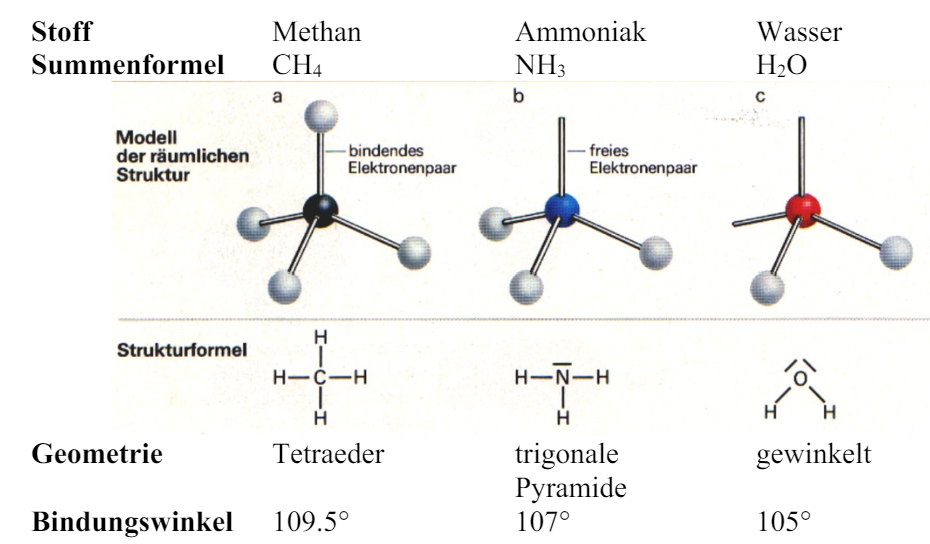
\includegraphics[height=4cm]{pictures/Winkel.png}
    \end{center}
\subsection{Löslichkeit}
    Die Löslichkeit von Salzen hängt von ihrer Bildungsstärke ab. Je grösser die Ladung der Ionen und je grösser die Ionen desto schlechter sind sie in Wasser löslich.
    \begin{center}
    \includegraphics[height=2cm]{pictures/Löslichkeit.png}
    \end{center}